% Fig.4: raw eBPF instruction counts per filter, Kunai vs cbpfc.
% Data source: benchmark/results/b1_insns.csv (filterset_test.go F1-F10).
% cbpfc bars exist only where pcap-filter can express the filter
% (F1-F4, F6); F5 and F7-F10 are Kunai-only.
% Build: pdflatex fig_insns.tex  ->  fig_insns.pdf
\documentclass[tikz]{standalone}
\usepackage{pgfplots}
\pgfplotsset{compat=1.18}
\begin{document}
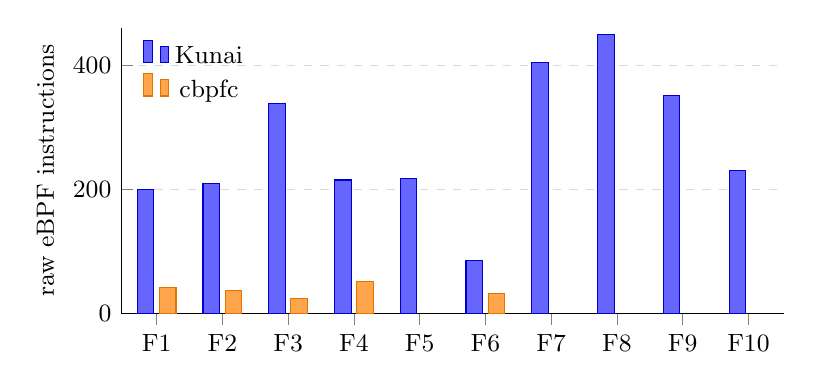
\begin{tikzpicture}
\begin{axis}[
    ybar,
    bar width=6pt,
    width=10cm,
    height=5.2cm,
    ymin=0,
    ymax=460,
    ylabel={raw eBPF instructions},
    symbolic x coords={F1,F2,F3,F4,F5,F6,F7,F8,F9,F10},
    xtick=data,
    ymajorgrids,
    major grid style={dashed, gray!30},
    axis x line*=bottom,
    axis y line*=left,
    enlarge x limits=0.06,
    legend style={at={(0.02,0.98)}, anchor=north west, draw=none, fill=none, font=\small},
    tick label style={font=\small},
    label style={font=\small},
]
\addplot+[fill=blue!60, draw=blue!80!black] coordinates {
    (F1,199) (F2,209) (F3,338) (F4,215) (F5,217)
    (F6,85) (F7,405) (F8,450) (F9,351) (F10,231)
};
\addplot+[fill=orange!70, draw=orange!90!black] coordinates {
    (F1,42) (F2,36) (F3,23) (F4,51) (F6,31)
};
\legend{Kunai, cbpfc}
\end{axis}
\end{tikzpicture}
\end{document}
